\renewcommand{\arraystretch}{1.5}
\begin{figure}[h]
  \centering
  \begin{tabular}{m{3cm}m{12cm}}
  \toprule
  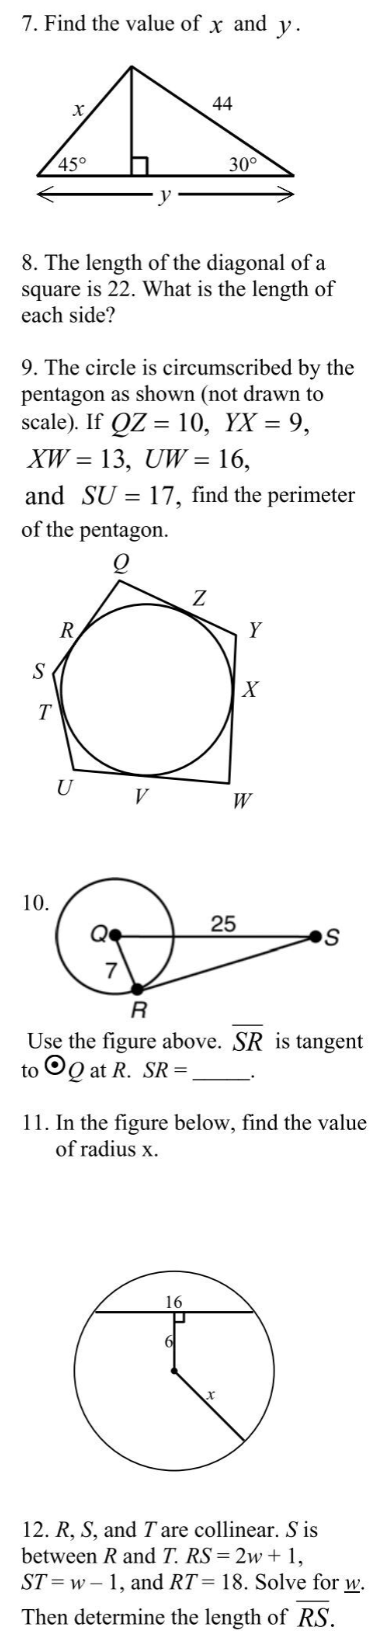
\includegraphics[width=3cm]{figures/example/example7.png} & 
  {\textbf{Instruction:} answer all the questions.\par
  \textbf{\mimovlrl{}:} \texttt{<think>...</think>}
\begin{enumerate}
\item Problem 7  
To find \( x \) and \( y \), we analyze the two right triangles formed by the height:  

- **Right triangle (30° angle)**:  
  Hypotenuse = 44. The height \( h \) (opposite 30°) is \( 44 \cdot \sin(30^\circ) = 44 \cdot 0.5 = 22 \).  
  The base segment \( y \) (adjacent to 30°) is \( 44 \cdot \cos(30^\circ) = 44 \cdot \frac{\sqrt{3}}{2} = 22\sqrt{3} \).  

- **Right triangle (45° angle)**:  
  This is a 45-45-90 triangle, so legs are equal. The height \( h = 22 \), so the other leg (left base segment) is also 22.  
  Hypotenuse \( x \) (45-45-90 ratio: leg \( \cdot \sqrt{2} \)) is \( 22\sqrt{2} \).  

\item Problem 8  
For a square with diagonal \( d = 22 \), the side length \( s \) relates to the diagonal by \( d = s\sqrt{2} \). Solving for \( s \):  
\( s = \frac{d}{\sqrt{2}} = \frac{22}{\sqrt{2}} = 11\sqrt{2} \) (rationalizing the denominator).  

\item Problem 9  
A pentagon circumscribed about a circle (tangential pentagon) has the property that the sum of the lengths of all sides equals \( 2 \times \) the sum of the tangent segments from each vertex. However, since the problem provides the side lengths \( QZ = 10 \), \( YX = 9 \), \( XW = 13 \), \( UW = 16 \), \( SU = 17 \), and the pentagon is tangential, the perimeter is the sum of these sides (as they represent the sides of the pentagon).  

Perimeter \( = 10 + 9 + 13 + 16 + 17 = 65 \).  

\item Problem 10  
\( \overline{SR} \) is tangent to \( \odot Q \) at \( R \), so \( QR \perp SR \) (tangent is perpendicular to radius). Thus, \( \triangle QRS \) is a right triangle with \( QR = 7 \) (radius) and \( QS = 25 \) (hypotenuse). By the Pythagorean theorem:  
\( SR = \sqrt{QS^2 - QR^2} = \sqrt{25^2 - 7^2} = \sqrt{625 - 49} = \sqrt{576} = 24 \)  

\item Problem 11  
A perpendicular from the circle’s center to a chord bisects the chord. The chord length is 16, so half the chord is \( \frac{16}{2} = 8 \). The distance from the center to the chord is 6, forming a right triangle with legs 6 and 8, and hypotenuse \( x \) (radius). By the Pythagorean theorem:  
\( x = \sqrt{6^2 + 8^2} = \sqrt{36 + 64} = \sqrt{100} = 10 \)   

\item Problem 12  
Since \( R, S, T \) are collinear and \( S \) is between \( R \) and \( T \), \( RS + ST = RT \). Substitute \( RS = 2w + 1 \), \( ST = w - 1 \), and \( RT = 18 \):  
\[ (2w + 1) + (w - 1) = 18 \]  
Simplify: \( 3w = 18 \implies w = 6 \).  
Substitute \( w = 6 \) into \( RS \):  
\( RS = 2(6) + 1 = 13 \) 
\end{enumerate}

\textbf{Final Answers}
7. \( x = 22\sqrt{2} \), \( y = 22\sqrt{3} \)  
8. \( 11\sqrt{2} \)  
9. \( 65 \)  
10. \( 24 \)  
11. \( 10 \)  
12. \( w = 6 \), \( \overline{RS} = 13 \)
} \\
  \bottomrule
  \end{tabular}
\caption{Example of \mimovlrl{} solving multiple geometry problems.}
\label{fig:case4}
\end{figure}
\renewcommand{\arraystretch}{1}

\clearpage
